% Options for packages loaded elsewhere
\PassOptionsToPackage{unicode}{hyperref}
\PassOptionsToPackage{hyphens}{url}
%
\documentclass[
  ignorenonframetext,
]{beamer}
\usepackage{pgfpages}
\setbeamertemplate{caption}[numbered]
\setbeamertemplate{caption label separator}{: }
\setbeamercolor{caption name}{fg=normal text.fg}
\beamertemplatenavigationsymbolsempty
% Prevent slide breaks in the middle of a paragraph
\widowpenalties 1 10000
\raggedbottom
\setbeamertemplate{part page}{
  \centering
  \begin{beamercolorbox}[sep=16pt,center]{part title}
    \usebeamerfont{part title}\insertpart\par
  \end{beamercolorbox}
}
\setbeamertemplate{section page}{
  \centering
  \begin{beamercolorbox}[sep=12pt,center]{part title}
    \usebeamerfont{section title}\insertsection\par
  \end{beamercolorbox}
}
\setbeamertemplate{subsection page}{
  \centering
  \begin{beamercolorbox}[sep=8pt,center]{part title}
    \usebeamerfont{subsection title}\insertsubsection\par
  \end{beamercolorbox}
}
\AtBeginPart{
  \frame{\partpage}
}
\AtBeginSection{
  \ifbibliography
  \else
    \frame{\sectionpage}
  \fi
}
\AtBeginSubsection{
  \frame{\subsectionpage}
}
\usepackage{amsmath,amssymb}
\usepackage{lmodern}
\usepackage{iftex}
\ifPDFTeX
  \usepackage[T1]{fontenc}
  \usepackage[utf8]{inputenc}
  \usepackage{textcomp} % provide euro and other symbols
\else % if luatex or xetex
  \usepackage{unicode-math}
  \defaultfontfeatures{Scale=MatchLowercase}
  \defaultfontfeatures[\rmfamily]{Ligatures=TeX,Scale=1}
\fi
\usetheme[]{Montpellier}
% Use upquote if available, for straight quotes in verbatim environments
\IfFileExists{upquote.sty}{\usepackage{upquote}}{}
\IfFileExists{microtype.sty}{% use microtype if available
  \usepackage[]{microtype}
  \UseMicrotypeSet[protrusion]{basicmath} % disable protrusion for tt fonts
}{}
\makeatletter
\@ifundefined{KOMAClassName}{% if non-KOMA class
  \IfFileExists{parskip.sty}{%
    \usepackage{parskip}
  }{% else
    \setlength{\parindent}{0pt}
    \setlength{\parskip}{6pt plus 2pt minus 1pt}}
}{% if KOMA class
  \KOMAoptions{parskip=half}}
\makeatother
\usepackage{xcolor}
\IfFileExists{xurl.sty}{\usepackage{xurl}}{} % add URL line breaks if available
\IfFileExists{bookmark.sty}{\usepackage{bookmark}}{\usepackage{hyperref}}
\hypersetup{
  hidelinks,
  pdfcreator={LaTeX via pandoc}}
\urlstyle{same} % disable monospaced font for URLs
\newif\ifbibliography
\usepackage{color}
\usepackage{fancyvrb}
\newcommand{\VerbBar}{|}
\newcommand{\VERB}{\Verb[commandchars=\\\{\}]}
\DefineVerbatimEnvironment{Highlighting}{Verbatim}{commandchars=\\\{\}}
% Add ',fontsize=\small' for more characters per line
\usepackage{framed}
\definecolor{shadecolor}{RGB}{248,248,248}
\newenvironment{Shaded}{\begin{snugshade}}{\end{snugshade}}
\newcommand{\AlertTok}[1]{\textcolor[rgb]{0.94,0.16,0.16}{#1}}
\newcommand{\AnnotationTok}[1]{\textcolor[rgb]{0.56,0.35,0.01}{\textbf{\textit{#1}}}}
\newcommand{\AttributeTok}[1]{\textcolor[rgb]{0.77,0.63,0.00}{#1}}
\newcommand{\BaseNTok}[1]{\textcolor[rgb]{0.00,0.00,0.81}{#1}}
\newcommand{\BuiltInTok}[1]{#1}
\newcommand{\CharTok}[1]{\textcolor[rgb]{0.31,0.60,0.02}{#1}}
\newcommand{\CommentTok}[1]{\textcolor[rgb]{0.56,0.35,0.01}{\textit{#1}}}
\newcommand{\CommentVarTok}[1]{\textcolor[rgb]{0.56,0.35,0.01}{\textbf{\textit{#1}}}}
\newcommand{\ConstantTok}[1]{\textcolor[rgb]{0.00,0.00,0.00}{#1}}
\newcommand{\ControlFlowTok}[1]{\textcolor[rgb]{0.13,0.29,0.53}{\textbf{#1}}}
\newcommand{\DataTypeTok}[1]{\textcolor[rgb]{0.13,0.29,0.53}{#1}}
\newcommand{\DecValTok}[1]{\textcolor[rgb]{0.00,0.00,0.81}{#1}}
\newcommand{\DocumentationTok}[1]{\textcolor[rgb]{0.56,0.35,0.01}{\textbf{\textit{#1}}}}
\newcommand{\ErrorTok}[1]{\textcolor[rgb]{0.64,0.00,0.00}{\textbf{#1}}}
\newcommand{\ExtensionTok}[1]{#1}
\newcommand{\FloatTok}[1]{\textcolor[rgb]{0.00,0.00,0.81}{#1}}
\newcommand{\FunctionTok}[1]{\textcolor[rgb]{0.00,0.00,0.00}{#1}}
\newcommand{\ImportTok}[1]{#1}
\newcommand{\InformationTok}[1]{\textcolor[rgb]{0.56,0.35,0.01}{\textbf{\textit{#1}}}}
\newcommand{\KeywordTok}[1]{\textcolor[rgb]{0.13,0.29,0.53}{\textbf{#1}}}
\newcommand{\NormalTok}[1]{#1}
\newcommand{\OperatorTok}[1]{\textcolor[rgb]{0.81,0.36,0.00}{\textbf{#1}}}
\newcommand{\OtherTok}[1]{\textcolor[rgb]{0.56,0.35,0.01}{#1}}
\newcommand{\PreprocessorTok}[1]{\textcolor[rgb]{0.56,0.35,0.01}{\textit{#1}}}
\newcommand{\RegionMarkerTok}[1]{#1}
\newcommand{\SpecialCharTok}[1]{\textcolor[rgb]{0.00,0.00,0.00}{#1}}
\newcommand{\SpecialStringTok}[1]{\textcolor[rgb]{0.31,0.60,0.02}{#1}}
\newcommand{\StringTok}[1]{\textcolor[rgb]{0.31,0.60,0.02}{#1}}
\newcommand{\VariableTok}[1]{\textcolor[rgb]{0.00,0.00,0.00}{#1}}
\newcommand{\VerbatimStringTok}[1]{\textcolor[rgb]{0.31,0.60,0.02}{#1}}
\newcommand{\WarningTok}[1]{\textcolor[rgb]{0.56,0.35,0.01}{\textbf{\textit{#1}}}}
\setlength{\emergencystretch}{3em} % prevent overfull lines
\providecommand{\tightlist}{%
  \setlength{\itemsep}{0pt}\setlength{\parskip}{0pt}}
\setcounter{secnumdepth}{-\maxdimen} % remove section numbering
%\documentclass[unicode,10pt]{beamer}% 'unicode'が必要
\usepackage{luatexja}% 日本語を使う場合は必須
%\usepackage[japanese]{babel}	
%\usefonttheme[onlymath]{serif}
%\usepackage[T1]{fontenc} %これを使うと、ギリシャ文字が出ない
%\usepackage{textcomp}
%\usepackage[scale=1.0]{tgheros} % Sans serif font
%\usepackage[scaled]{beramono} % Monospace font
%\usepackage{luatexja-otf}
%\renewcommand{\kanjifamilydefault}{\gtdefault}
%\usepackage[haranoaji]{luatexja-preset}

% スライド番号の表示 %%%%%%%%%%%%%%%%%%%
\makeatletter
\setbeamertemplate{footline}{%
  \leavevmode%
  \hbox{%
  \begin{beamercolorbox}[wd=.5\paperwidth,ht=2.25ex,dp=1ex,right]{date in head/foot}%
    \insertframenumber{} \hspace*{2ex} % new version without total frames
  \end{beamercolorbox}}%
  \vskip0pt%
}
\makeatother
% スライド番号の表示 %%%%%%%%%%%%%%%%%%%
\ifLuaTeX
  \usepackage{selnolig}  % disable illegal ligatures
\fi

\title{第2章: 因果関係\\
(2.5. 観察研究)}
\subtitle{今井耕介 著\\
『社会科学のためのデータ分析入門 (QSS)』}
\author{}
\date{\vspace{-2.5em}2026-03-09}

\begin{document}
\frame{\titlepage}

\hypertarget{ux89b3ux5bdfux7814ux7a76-observational-studies}{%
\section{2.5 観察研究 (Observational
Studies)}\label{ux89b3ux5bdfux7814ux7a76-observational-studies}}

\begin{frame}{観察研究とは}
\protect\hypertarget{ux89b3ux5bdfux7814ux7a76ux3068ux306f}{}
\begin{itemize}
\tightlist
\item
  \textbf{観察研究}: 研究者が処置を無作為に割り当て\textbf{ない}研究。

  \begin{itemize}
  \tightlist
  \item
    実世界のデータ（自然に発生したデータ）を分析する。
  \end{itemize}
\item
  \textbf{課題}: \textbf{交絡バイアス} (Confounding Bias)。

  \begin{itemize}
  \tightlist
  \item
    処置群と対照群が、処置以外の要因（共変量）についても異なっている可能性がある。
  \end{itemize}
\item
  \textbf{解決策のデザイン}:

  \begin{enumerate}
  \tightlist
  \item
    \textbf{前後比較} (Before-and-After) デザイン
  \item
    \textbf{差の差} (Difference-in-Differences: DiD) デザイン
  \end{enumerate}
\end{itemize}
\end{frame}

\hypertarget{ux6700ux4f4eux8cc3ux91d1ux3068ux96c7ux7528}{%
\section{2.5.1
最低賃金と雇用}\label{ux6700ux4f4eux8cc3ux91d1ux3068ux96c7ux7528}}

\begin{frame}[fragile]{カード＝クルーガー研究 (1994)}
\protect\hypertarget{ux30abux30fcux30c9ux30afux30ebux30fcux30acux30fcux7814ux7a76-1994}{}
\begin{itemize}
\tightlist
\item
  \textbf{問い}: 最低賃金を引き上げると、雇用（失業）はどう変化するか？
\item
  \textbf{事例}:

  \begin{itemize}
  \tightlist
  \item
    1992年にニュージャージー州 (NJ) が最低賃金を引き上げた。
  \item
    隣接するペンシルベニア州 (PA) は引き上げなかった。
  \end{itemize}
\item
  \textbf{データ}: 両州のファストフード店の雇用データ
  (\texttt{minwage.csv})。
\end{itemize}
\end{frame}

\begin{frame}[fragile]{minwage データの読み込み (1)}
\protect\hypertarget{minwage-ux30c7ux30fcux30bfux306eux8aadux307fux8fbcux307f-1}{}
\begin{itemize}
\tightlist
\item
  カード＝クルーガー研究のデータをRに読み込みます。
\end{itemize}

\scriptsize

\begin{Shaded}
\begin{Highlighting}[]
\CommentTok{\# 1. ローカルに保存したminwageデータの読み込み（推奨）}
\NormalTok{minwage }\OtherTok{\textless{}{-}} \FunctionTok{read.csv}\NormalTok{(}\StringTok{"minwage.csv"}\NormalTok{)}

\CommentTok{\# （参考）URLから直接読み込むことも可能}
\CommentTok{\# minwage \textless{}{-} read.csv("https://ayumu{-}tanaka.github.io/QSS/QSS\_Data/minwage.csv")}

\CommentTok{\# 2. データの次元（行数と列数）を確認}
\FunctionTok{dim}\NormalTok{(minwage)}
\end{Highlighting}
\end{Shaded}

\begin{verbatim}
## [1] 358   8
\end{verbatim}

\normalsize
\end{frame}

\begin{frame}[fragile]{州別のデータ分割 (2)}
\protect\hypertarget{ux5ddeux5225ux306eux30c7ux30fcux30bfux5206ux5272-2}{}
\begin{itemize}
\tightlist
\item
  ニュージャージー州 (NJ) とペンシルベニア州 (PA)
  にデータを分け、規模を確認します。
\end{itemize}

\scriptsize

\begin{Shaded}
\begin{Highlighting}[]
\CommentTok{\# 1. location列が "PA" かどうかで判定して抽出}
\NormalTok{minwageNJ }\OtherTok{\textless{}{-}} \FunctionTok{subset}\NormalTok{(minwage, }\AttributeTok{subset =}\NormalTok{ (location }\SpecialCharTok{!=} \StringTok{"PA"}\NormalTok{))}
\NormalTok{minwagePA }\OtherTok{\textless{}{-}} \FunctionTok{subset}\NormalTok{(minwage, }\AttributeTok{subset =}\NormalTok{ (location }\SpecialCharTok{==} \StringTok{"PA"}\NormalTok{))}

\CommentTok{\# 2. データの規模を確認}
\FunctionTok{dim}\NormalTok{(minwageNJ) }\CommentTok{\# NJの店舗数}
\end{Highlighting}
\end{Shaded}

\begin{verbatim}
## [1] 291   8
\end{verbatim}

\begin{Shaded}
\begin{Highlighting}[]
\FunctionTok{dim}\NormalTok{(minwagePA) }\CommentTok{\# PAの店舗数}
\end{Highlighting}
\end{Shaded}

\begin{verbatim}
## [1] 67  8
\end{verbatim}

\normalsize
\end{frame}

\begin{frame}[fragile]{賃金引き上げの確認}
\protect\hypertarget{ux8cc3ux91d1ux5f15ux304dux4e0aux3052ux306eux78baux8a8d}{}
\begin{itemize}
\tightlist
\item
  実際にNJ州だけで賃金が上がったかを確認します。
\end{itemize}

\scriptsize

\begin{Shaded}
\begin{Highlighting}[]
\CommentTok{\# 時給が $5.05（以前の最低賃金）未満の店舗の割合を計算}
\CommentTok{\# 引き上げ前 (wageBefore)}
\FunctionTok{mean}\NormalTok{(minwageNJ}\SpecialCharTok{$}\NormalTok{wageBefore }\SpecialCharTok{\textless{}} \FloatTok{5.05}\NormalTok{) }
\end{Highlighting}
\end{Shaded}

\begin{verbatim}
## [1] 0.9106529
\end{verbatim}

\begin{Shaded}
\begin{Highlighting}[]
\FunctionTok{mean}\NormalTok{(minwagePA}\SpecialCharTok{$}\NormalTok{wageBefore }\SpecialCharTok{\textless{}} \FloatTok{5.05}\NormalTok{)}
\end{Highlighting}
\end{Shaded}

\begin{verbatim}
## [1] 0.9402985
\end{verbatim}

\begin{Shaded}
\begin{Highlighting}[]
\CommentTok{\# 引き上げ後 (wageAfter)}
\FunctionTok{mean}\NormalTok{(minwageNJ}\SpecialCharTok{$}\NormalTok{wageAfter }\SpecialCharTok{\textless{}} \FloatTok{5.05}\NormalTok{)  }\CommentTok{\# NJは 0 に近いはず}
\end{Highlighting}
\end{Shaded}

\begin{verbatim}
## [1] 0.003436426
\end{verbatim}

\begin{Shaded}
\begin{Highlighting}[]
\FunctionTok{mean}\NormalTok{(minwagePA}\SpecialCharTok{$}\NormalTok{wageAfter }\SpecialCharTok{\textless{}} \FloatTok{5.05}\NormalTok{)  }\CommentTok{\# PAは高いままのはず}
\end{Highlighting}
\end{Shaded}

\begin{verbatim}
## [1] 0.9552239
\end{verbatim}

\normalsize
\end{frame}

\hypertarget{ux4ea4ux7d61ux30d0ux30a4ux30a2ux30b9-confounding-bias}{%
\section{2.5.2 交絡バイアス (Confounding
Bias)}\label{ux4ea4ux7d61ux30d0ux30a4ux30a2ux30b9-confounding-bias}}

\begin{frame}[fragile]{単純な比較の危険性}
\protect\hypertarget{ux5358ux7d14ux306aux6bd4ux8f03ux306eux5371ux967aux6027}{}
\begin{itemize}
\tightlist
\item
  引き上げ後のNJ州とPA州の雇用率を単純に比較します。
\end{itemize}

\scriptsize

\begin{Shaded}
\begin{Highlighting}[]
\CommentTok{\# フルタイム雇用率 (fullPropAfter) を計算}
\CommentTok{\# フルタイム数 / (フルタイム数 + パートタイム数)}
\NormalTok{minwageNJ}\SpecialCharTok{$}\NormalTok{fullPropAfter }\OtherTok{\textless{}{-}}\NormalTok{ minwageNJ}\SpecialCharTok{$}\NormalTok{fullAfter }\SpecialCharTok{/} 
\NormalTok{    (minwageNJ}\SpecialCharTok{$}\NormalTok{fullAfter }\SpecialCharTok{+}\NormalTok{ minwageNJ}\SpecialCharTok{$}\NormalTok{partAfter)}
\NormalTok{minwagePA}\SpecialCharTok{$}\NormalTok{fullPropAfter }\OtherTok{\textless{}{-}}\NormalTok{ minwagePA}\SpecialCharTok{$}\NormalTok{fullAfter }\SpecialCharTok{/} 
\NormalTok{    (minwagePA}\SpecialCharTok{$}\NormalTok{fullAfter }\SpecialCharTok{+}\NormalTok{ minwagePA}\SpecialCharTok{$}\NormalTok{partAfter)}

\CommentTok{\# NJ州とPA州の平均の差を計算}
\FunctionTok{mean}\NormalTok{(minwageNJ}\SpecialCharTok{$}\NormalTok{fullPropAfter) }\SpecialCharTok{{-}} \FunctionTok{mean}\NormalTok{(minwagePA}\SpecialCharTok{$}\NormalTok{fullPropAfter)}
\end{Highlighting}
\end{Shaded}

\begin{verbatim}
## [1] 0.04811886
\end{verbatim}

\normalsize

\begin{itemize}
\tightlist
\item
  \textbf{問題}:
  NJとPAは州そのものが異なる（経済状況など）。この差が「最低賃金」によるものか「州の違い」によるものか区別できない。これが\textbf{交絡}である。
\end{itemize}
\end{frame}

\hypertarget{ux524dux5f8cux6bd4ux8f03ux3068ux5deeux306eux5dee-did-ux30c7ux30b6ux30a4ux30f3}{%
\section{2.5.3 前後比較と差の差 (DiD)
デザイン}\label{ux524dux5f8cux6bd4ux8f03ux3068ux5deeux306eux5dee-did-ux30c7ux30b6ux30a4ux30f3}}

\begin{frame}[fragile]{1. 前後比較 (Before-and-After) デザイン}
\protect\hypertarget{ux524dux5f8cux6bd4ux8f03-before-and-after-ux30c7ux30b6ux30a4ux30f3}{}
\begin{itemize}
\tightlist
\item
  同じNJ州の中で、引き上げ前と後を比較します。
\end{itemize}

\scriptsize

\begin{Shaded}
\begin{Highlighting}[]
\CommentTok{\# NJ州の引き上げ前の雇用率を計算}
\NormalTok{minwageNJ}\SpecialCharTok{$}\NormalTok{fullPropBefore }\OtherTok{\textless{}{-}}\NormalTok{ minwageNJ}\SpecialCharTok{$}\NormalTok{fullBefore }\SpecialCharTok{/} 
\NormalTok{    (minwageNJ}\SpecialCharTok{$}\NormalTok{fullBefore }\SpecialCharTok{+}\NormalTok{ minwageNJ}\SpecialCharTok{$}\NormalTok{partBefore)}

\CommentTok{\# 前後の差を計算}
\NormalTok{NJdiff }\OtherTok{\textless{}{-}} \FunctionTok{mean}\NormalTok{(minwageNJ}\SpecialCharTok{$}\NormalTok{fullPropAfter) }\SpecialCharTok{{-}} \FunctionTok{mean}\NormalTok{(minwageNJ}\SpecialCharTok{$}\NormalTok{fullPropBefore)}
\NormalTok{NJdiff}
\end{Highlighting}
\end{Shaded}

\begin{verbatim}
## [1] 0.02387474
\end{verbatim}

\normalsize

\begin{itemize}
\tightlist
\item
  \textbf{問題}:
  時間の経過とともに、最低賃金とは無関係に経済全体が変化した可能性がある。
\end{itemize}
\end{frame}

\begin{frame}[fragile]{2. 差の差 (Difference-in-Differences: DiD)}
\protect\hypertarget{ux5deeux306eux5dee-difference-in-differences-did}{}
\begin{itemize}
\tightlist
\item
  \textbf{アイデア}:
  NJ州の変化から、PA州（対照群）で起きた変化（自然なトレンド）を差し引く。
\item
  \textbf{数式}:
  \(\text{DiD} = (NJ_{\text{after}} - NJ_{\text{before}}) - (PA_{\text{after}} - PA_{\text{before}})\)
\end{itemize}

\scriptsize

\begin{Shaded}
\begin{Highlighting}[]
\CommentTok{\# PA州の引き上げ前後の雇用率の変化を計算}
\NormalTok{minwagePA}\SpecialCharTok{$}\NormalTok{fullPropBefore }\OtherTok{\textless{}{-}}\NormalTok{ minwagePA}\SpecialCharTok{$}\NormalTok{fullBefore }\SpecialCharTok{/} 
\NormalTok{    (minwagePA}\SpecialCharTok{$}\NormalTok{fullBefore }\SpecialCharTok{+}\NormalTok{ minwagePA}\SpecialCharTok{$}\NormalTok{partBefore)}
\NormalTok{PAdiff }\OtherTok{\textless{}{-}} \FunctionTok{mean}\NormalTok{(minwagePA}\SpecialCharTok{$}\NormalTok{fullPropAfter) }\SpecialCharTok{{-}} \FunctionTok{mean}\NormalTok{(minwagePA}\SpecialCharTok{$}\NormalTok{fullPropBefore)}

\CommentTok{\# 差の差 (DiD) を計算}
\NormalTok{NJdiff }\SpecialCharTok{{-}}\NormalTok{ PAdiff}
\end{Highlighting}
\end{Shaded}

\begin{verbatim}
## [1] 0.06155831
\end{verbatim}

\normalsize

\begin{itemize}
\tightlist
\item
  \textbf{結論}:
  最低賃金引き上げ後、NJ州のフルタイム雇用率はPA州に比べて相対的に約 6.2
  パーセントポイント上昇した（雇用は減らなかった）。
\end{itemize}
\end{frame}

\begin{frame}{差の差 (DiD) の概念図}
\protect\hypertarget{ux5deeux306eux5dee-did-ux306eux6982ux5ff5ux56f3}{}
\begin{center}
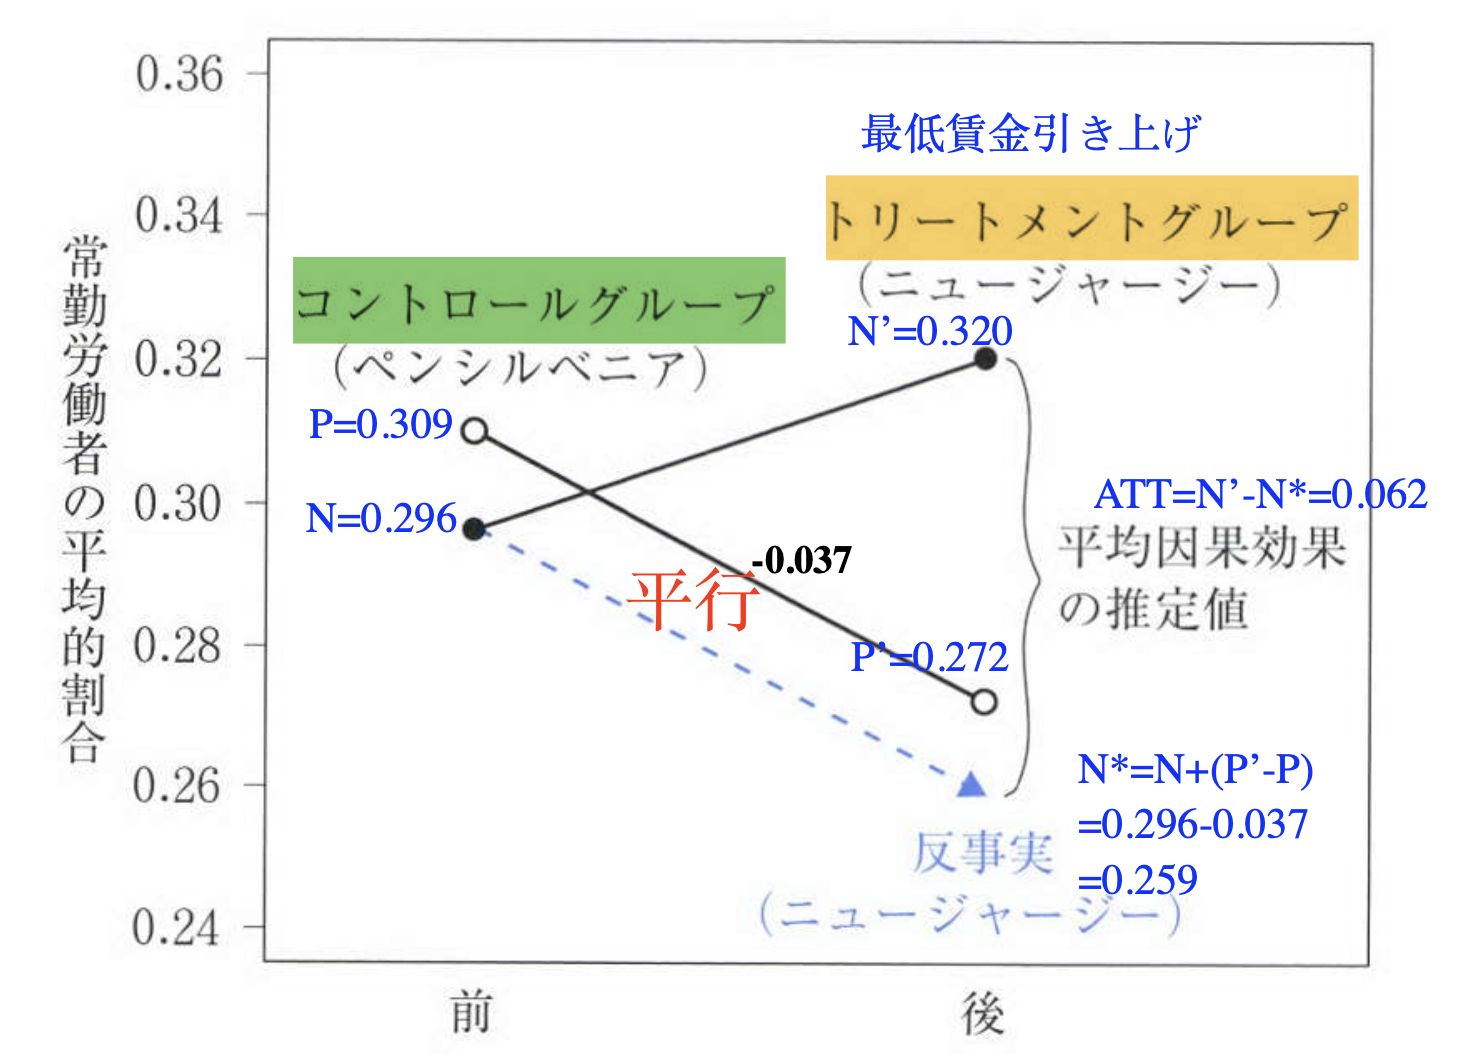
\includegraphics[width=0.8\textwidth]{fig2_2.png}
\end{center}

\begin{itemize}
\tightlist
\item
  \textbf{平行トレンド仮定}:
  もし処置がなければ、処置群と対照群は同じトレンドを辿るという仮定が重要。
\end{itemize}
\end{frame}

\hypertarget{ux307eux3068ux3081}{%
\section{2.5.4 まとめ}\label{ux307eux3068ux3081}}

\begin{frame}[fragile]{このセクションのまとめ}
\protect\hypertarget{ux3053ux306eux30bbux30afux30b7ux30e7ux30f3ux306eux307eux3068ux3081}{}
\begin{itemize}
\tightlist
\item
  \textbf{観察研究}:
  現実世界のデータには交絡因子が潜んでいるため、慎重なデザインが必要。
\item
  \textbf{交絡バイアス}:
  処置以外の要因が結果に影響を与え、因果推論を妨げること。
\item
  \textbf{差の差 (DiD) デザイン}:

  \begin{itemize}
  \tightlist
  \item
    処置群の変化から、比較可能な対照群の変化を差し引くことで、共通のトレンドを制御する。
  \item
    社会科学において非常に多用される強力な手法。
  \end{itemize}
\item
  \textbf{Rの操作}:

  \begin{itemize}
  \tightlist
  \item
    複雑な数式（雇用率の計算など）をデータフレームの列同士の演算で行う。
  \item
    \texttt{subset()} を用いた州や時期の切り分け。
  \end{itemize}
\end{itemize}
\end{frame}

\end{document}
